\chapter{Diskussion}
\label{sec:diskussion}
In diesem Abschnitt des Protokolls werden nun die Ergebnisse des Abschnittes \ref{sec:ergebnisse} diskutiert und ausgewertet.\\

%Sedimentationsverhalten

Das Sedimentationsverhalten der Probe 1 unterscheidet sich signifikant von dem der Proben 2 und 3. Die Probe 1 enthält einen sehr großen Anteil an Schwebstoffen\linebreak (siehe Tab. \ref{tab:filter}) in grobflockiger Form. Diese setzen sich aufgrund ihrer Größe und Zahl zügig auf ein großes Absetzvolumen ab. Dabei entstehen nur zwei erkennbare Zonen. Die erste Zone ist die rasch wachsende Klarphase im oberen Bereich. Die zweite Zone ist die Sedimentationszone, welche von der Trennschicht bis zum Boden des Imhofftrichters reicht. Eine Kompressionszone deutet sich etwa nach einer Absetzdauer von 10 Minuten an, verglichen mit Abb. \ref{dia:sedimentation_1} und Abb. \ref{fig:Absetzphasen-merkel1971}.\\
 \begin{figure}[h!]
\centering
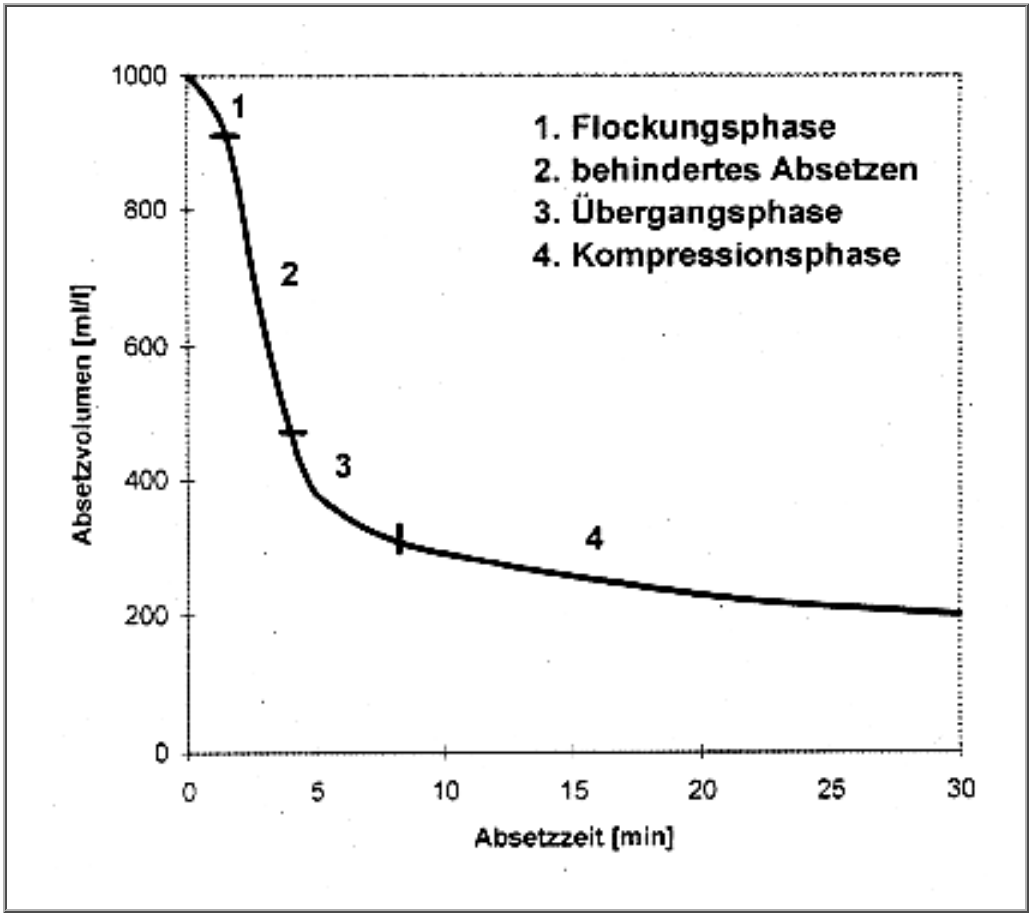
\includegraphics[width=0.6\linewidth]{img/Absetzphasen_merkel1971}
\caption[Zeitliche Phasen des Absetzvorganges]{Zeitliche Phasen des Absetzvorganges \cite{merkel1971untersuchungen}}
\label{fig:Absetzphasen-merkel1971}
\end{figure}
\FloatBarrier



Ganz im Gegensatz dazu bildet die Probe 2  eine recht dünne, klare Schicht im aller obersten Bereich. Darunter folgt eine sich über den Versuchszeitraum kaum verändernde Trübe. Am Boden schließlich sammelt sich das abgesetzte Material. Es handelte sich dabei um die Art der Schichtung, bei welcher sich aus der Trübe eine Setimentationszone herausbildet. Aus der Probe 2 fallen vereinzelte Partikel etwas zügiger aus und bilden einen geringen Bodensatz. Somit ist das Sedimentationsverhalten der Probe 2 verglichen mit der Probe 1 in der Beschaffenheit der Abwasserproben unterschiedlich.
Die Struktur der Feststoffe in Probe 1 enthält einen klassischen "`Schlamm"', während die Proben 2 und 3 eher durch feine Schwebstoffe verunreinigt sind. Das hat zur Folge, dass für die Auswertung des Sedimentationsverhalten, der untersuchten Abwasserproben, lediglich Probe 1 nach der Abb. \ref{fig:Absetzphasen-merkel1971} charakterisiert werden kann. 
\newpage
Die Proben 2 und 3 benötigen anderweitige Methoden der Auswertung des Sedimentationsverhaltens. Ähnlich verhält es sich mit den Ergebnissen des Schlammvolumenindexes (SVI), da in den Proben effektiv nicht von einem zusammenhängenden Schlamm gesprochen werden kann.\\
Das hat zur Folge, dass für die Proben 2 und 3 eher der beginnende Bodensatz betrachtet wird. Dieser bildete sich in beiden Proben vom Boden beginnend langsam bis zu einem Volumen von wenigen Millilitern.
Bei der Probe 1 setzten sich  die Schwebstoffe gleichzeitig und wie als einzige Masse von oben beginnend nach unten ab. Somit ergeben sich unterschiedliche Wertebereiche der Absetzvolumen zwischen der Probe 1 und den Proben 2 und 3, welche in den Graphen, der Abb. \ref{dia:sedimentation_1} und Abb. \ref{dia:sedimentation_12} getrennt dargestellt sind.\\
Als Schlussfolgerung dazu ließe sich Probe 1 hervorragend in einem Absetzbecken trennen. Die Proben 2 und 3 brauchen für den selben Fortschritt ungemein länger. Die Verweilzeit von \SI{30}{\minute} könnte für ein spezifikationsgerechtes Absetzen im Einzelfall nicht ausreichen. In diesen Fällen schaffen Flockungsmittel Abhilfe durch Koagulation und dadurch erhöhte Absinkgeschwindigkeiten.\\


%Trockensubstanz und organische Trockensubstanz ist nicht als Auswertungspunkt gefragt

%Anorganische Trockensubstanz muss als Schlamm aus dem klärprozess ausgetragen werden, da es sich sonst im System anreichert. \cite[91]{rosenwinkelAnaerobtechnikAbwasserSchlamm2015}

%"'Bei der anaeroben Behandlung von Schlämmen (z. B. Klärschlammstabilisierung) wird üblicherweise die organische Trockenmasse des zugeführten Substrates als Bemessungsgröße für Anaerobreaktoren, und zwar über die Berechnung der organischen Raumbelastung, verwendet.

%Bei anderen Schlämmen (z. B. Abfälle aus der Nahrungsmittelindustrie) ist die organische Trockenmasse als Bemessungswert und Bezugswert für die zu erwartende Gasmenge nur bedingt geeignet."'




%Berechnen Sie für die Abwasserschlammproben den Schlammvolumenindex (SVI)! 
%Nach MOHLMANN gibt dieser das Volumen von 1 g Trockensubstanz des Belebtschlammes nach einer 
%Absetzzeit von 30 min an und stellt sich als Verhältnis spez. Volumen des abgesetzten Schlammes in 
%ml/1000ml und spez. Masse der Trockensubstanz in g/1000ml dar. 

Der Schlammvolumenindex wurde für die untersuchten Abwässer im Kapitel \ref{sec:ergebnisse} berechnet und die Ergebnisse in Tab. \ref{tab:svi} aufgeführt.
%Welche Aussage können Sie mit dem SVI für Ihre Proben machen?
Der Schlammvolumenindex SVI gibt Auskunft über das Absetzverhalten und die Absetzeigenschaften des Schlammes. Besonders wichtig ist er für die Einschätzung von Schlämmen aus der biologischen Abwasserbehandlung. 
Ein normaler Wert für den SVI liegt zwischen \SI{100}{\milli\liter\per\gram} und \SI{120}{\milli\liter\per\gram}. Ein höherer SVI deutet auf schlechtes Absetz- und Eindickverhalten hin. Ab etwa \SI{150}{\milli\liter\per\gram} gilt der Schlamm als Blähschlamm. Umso geringer die Werte sind, umso besser ist die Absetzbarkeit des Schlammes.\cite{Dr.ManfredNeupert.August2008}\\
Der errechnete SVI-Wert für die Probe 1 bewegt sich mit \SI{160}{\milli\liter\per\gram} in einem realistischen Wertebereich. Der Schlamm ist nach \cite{Dr.ManfredNeupert.August2008} als Blähschlamm einzustufen. Die SVI-Werte der Proben 2 und 3 stimmen nicht mit den beobachteten Absetzverhalten überein. Die SVI-Werte kleiner \SI{45}{\milli\liter\per\gram} sollten ein sehr schnelles Absetzen erwarten lassen. Ein Vergleich mit der Abb. \ref{dia:sedimentation_12} ergibt, in Verbindung mit der erheblichen verbliebenen Trübheit der Wässer mit sichtbaren Feststoffpartikeln, ein gegenteiliges Bild. Der Schlammvolumenindex bezieht sich laut \cite{Dr.ManfredNeupert.August2008} nur auf Belebtschlamm. Die Proben 2 und 3 enthalten keinen Belebtschlamm, daher gilt lediglich der Messwert für Abwasserprobe 1 als plausibel. \\




%Die erhaltenen Analysenergebnisse sind tabellarisch und grafisch darzustellen.  
%%In Ergebnissen meiner meinung nach ausreichend erfolgt



%Was bedeuten CSB und BSB5 ? Erklären Sie die Merkmale und den Stellenwert beider Analysen.
Der $CSB$-Wert gibt an wie viel Sauerstoff von einem  starken chemischen Oxidationsmittel, wie etwa Kaliumdichromat, zur Oxidation aller im Wasser enthaltenen oxidierbaren Stoffe verbraucht wird. Neben den biologischen und organischen Stoffen werden zum Teil auch anorganische Verbindungen oxidiert. Darum liegt der $CSB$ in der Regel höher als der $BSB_5$.\\
Der $BSB_5$ gibt an wie viel Sauerstoff bei der biologischen Oxidation im Wasser befindlicher organischer Stoffe verbraucht wird. Nicht alle organischen Inhaltsstoffe können innerhalb der gewährten Zeit oxidiert werden. Außerdem werden circa 50\% der organischen Stoffe für das Wachstum der Mikroorganismen benötigt und ist somit nicht oxidiert.\cite[S.64]{rosenwinkelAnaerobtechnikAbwasserSchlamm2015} \\
\newpage
Die Angabe des $CSB$ und $BSB_5$ ermöglichen eine Einordnung der Abwässer hinsichtlich ihres Gehaltes an Biomasse (organischen Stoffen). Ins besondere bei der Abschätzung des Gefahrenpotentials des Abwassers für aquatische Ökosysteme sind der $CSB$, als auch der $BSB_5$, unerlässich.

 
%Warum beträgt die Dauer des BSB-Versuches 5 Tage? 
Die Dauer des BSB-Versuches beträgt fünf Tage, weil die verwendeten Mikroorganismen einige Zeit brauchen um sich entsprechend zu vermehren und die angebotene Biomasse zu verstoffwechseln. Fünf Tage sind außerdem eine realistische Verweilzeit für den Belebtschlamm in einer herkömmlichen Kläranlage.
\cite{KlaranlageROMPPThieme} \cite{SchlammalterROMPPThieme}
%Welches CSB/BSB5-Verhältnis besitzt biologisch gut abbaubares Abwasser, welches 
%„Problemwässer“? 

Bei kommunalen Abwässern ist ein Verhältnis von $CSB$ zu $BSB_5$ von etwa 2:1 häufig anzutreffen. 
Ist das Verhältnis $<2$ kann eine gute Abbaubarkeit erwartet werden. Bei Werten $> 2$ ist keine einfache Schlussfolgerung möglich. Das Wasser muss dann auf andere Arten untersucht werden.\\ "`Problemabwässer"' entstammen zumeist industriellen Quellen. Schadstoffe welche in der natürlichen Umgebung sehr  selten auftreten bedürfen zumeist spezieller Destruenten zum biologischen Abbau. Extrem große Verhältnisse von $CSB$ zu $BSB_5$ lassen darauf schließen, dass der $BSB_5$ sehr gering ausgeprägt ist. Geringe mikrobielle Aktivität hat demnach eine schlechte Abbaubarkeit zur Folge.\cite[S.64]{rosenwinkelAnaerobtechnikAbwasserSchlamm2015}
%Errechnen Sie das bestehende CSB/BSB5-Verhältnis und beurteilen Sie die 
%biologische Abbaubarkeit der einzelnen Proben. 
\vspace*{-3mm}
\begin{table}[h!]
	\centering
	\caption{Errechnete $CSB$-$BSB_5$-Verhältnisse }
	\label{tab:csb/bsb5}
	%\resizebox{10cm}{!}{
	\begin{tabulary}{1.2\textwidth}{l|C|C|C}
		\hline
		& \textbf{$CSB$} $\boldsymbol{\left[\si{\milli\gram\per\liter}\right]}$ & \textbf{$BSB_5$} $\boldsymbol{\left[\si{\milli\gram\per\liter}\right]}$&
		$\boldsymbol{\frac{CSB}{BSB_5}}$\\
		\hline

		Probe 1 & 575 & 254 &2,29\\
		Probe 2 & 486 & 252&1,93\\
		Probe 3 & 221 & 50&4,42\\
		\hline
	\end{tabulary}
	%}
\end{table}
\FloatBarrier
Die oben ergründete Bedeutung des $\frac{CSB}{BSB_5}$-Verhältnisses kann nun durch die in \mbox{Tab. \ref{tab:csb/bsb5}} Werte auf die getesteten Proben übertragen werden. Das $\frac{CSB}{BSB_5}$-Verhältnis der Probe 1 beträgt 2,29. Die Probe 1 gilt damit als mäßig gut abbaubar. Die \mbox{Probe 2} ist mit einem $\frac{CSB}{BSB_5}$-Verhältnis von 1,93 gut abbaubar. Eine schlechte Abbaubarkeit bescheinigt der Probe 3 ihr $\frac{CSB}{BSB_5}$-Verhältnis von 4,42.\\



%Die Werte sind den Mindestanforderungen für das Einleiten kommunaler Abwässer (GK 5; siehe 
%Anlage des Praktikumsheftes) gegenüberzustellen und zu diskutieren. 
Alle drei untersuchten Abwasserproben erreichen nicht die Mindestanforderungen für das Einleiten in den Vorfluter für die GK5. Dabei sticht die Probe 1 besonders heraus. Sie überschreitet den Grenzwert von \SI{75}{\milli\gram
	\per\liter} $CSB$ um das 7,6-Fache und den Grenzwert von \SI{15}{\milli\gram\per\liter} $BSB_5$ sogar um das knapp 17-Fache. Die Proben 2 und 3 können die Grenzwerte ebenfalls bei weitem nicht erfüllen, was in Abb. \ref{Balkendiagramm} dargestellt ist. 


%Ordnen Sie die Proben hinsichtlich ihres Belastungsgrades ein!
\newpage
Zur Einordnung der Proben hinsichtlich ihrer Belastung werden im Folgenden die in den Tabellen \ref{tab:absetzvol}, \ref{tab:filter}, \ref{tab:csb} und \ref{tab:bsb} aufgeführten Ergebnisse mit den Referenzwerten in Tabelle \ref{tab:komm} verglichen.
Die Proben 1 und 2 sind den $CSB$- und $BSB_5$-Werten nach mittelstark mit organischem Material belastet, wärend die Probe 3 als gering belastet einzustufen ist.
Weitere Merkmale für den Belastungsgrad stellen die Anteile absetzbarer und abfiltrierbarer Stoffe dar. Die Probe 3 mit \SI{90}{\milli\gram\per\liter} sehr gering belastet, wohingegen die Probe 2 mit \SI{210}{\milli\gram\per\liter} schon gering und die Probe 1 mit \SI{1319}{\milli\gram\per\liter} sehr stark belastet ist (siehe Abb. \ref{dia:abfilt}).
Die Betrachtung hinsichtlich absetzbarer Stoffe ergibt für die Probe 1 eine sehr starke Belastung mit einem Volumenanteil von \SI{210}{\milli\liter\per\liter} nach 30 Minuten. Von einer starken Belastung wird ab einem Wert von \SI{12}{\milli\liter\per\liter} ausgegangen. Die Proben 2 und 3 fallen bei \SI{2}{\milli\liter\per\liter} bis \SI{4}{\milli\liter\per\liter} beide unter die geringe Belastungsstufe (siehe Abb. \ref{dia:absetz}).\\


%Streichen Sie signifikante Unterschiede zwischen den einzelnen Proben heraus und schließen Sie auf 
%ihre Herkunft! 
Die Abwasserprobe enthält sehr große Mengen an abfiltrierbaren Stoffen. Ein hoher Anteil an Exkrementen könnte dazu geführt haben. Der Geruch lässt aber keinen Urinanteil erkennen. An Wänden in Kanälen bildet sich gern ein ausgeprägter Biofilm. Es könnte sich um Abwasser von der Reinigung dieser Wandbeläge handeln. Alternativ wäre eine Herkunft aus dem Belebungsbecken einer Kläranlage anzunehmen. Die Flocken lassen sich sowohl gut in schwebe halten als auch schnell absetzen. Die gröbsten Verunreinigungen sind in diesem Fall schon abgebaut und in Biomasse gebunden. Die hell-rotbraune Färbung des Schlamms findet sich auch in Lichtbildern von Klärbecken wieder.

Die Proben 2 und 3 lassen hingegen keine eindeutige Einordnung zu. Es handelt sich wahrscheinlich um Abwässer, wobei der niedrige $BSB_5$ der Probe 3 entweder auf eine bereits erfolgte Klärung, eine Industrielle Herkunft oder eine Schadstoffbelastung schließen lassen könnte. Die Probe 3 ist außerdem optisch heller als die Probe 2.
Die dunkle Färbung, die feine Beschaffenheit der Schwebstoffe und das Fehlen von Exkrementen, gepaart mit der mittelstarken Belastung an biologisch abbaubaren Substanzen könnten auf einen natürlichen Ursprung hinweisen. Beispiel hierfür könnte fauliges Wasser aus einem Sumpf oder Überschwemmungsgebiet sein.\\

%Geben Sie Empfehlungen zu einer anforderungsgerechten Behandlung der analysierten Proben. 

Die Proben 1 und 2 können einer kommunalen Kläranlage zugeführt werden. Der Gehalt absetzbarer und abfiltrierbarer Stoffe könnte damit behoben werden, das Abwasser vor dem Einleiten in die Kanalisation durch ein Absetzbecken zu leiten. Andernfalls muss auf eine ausreichende Spülung der Kanalrohre geachtet werden. Die Probe 3 sollte unter Umständen genauer analysiert werden um den Grund ihrer schlechten biologischen Abbaubarkeit heraus zu finden. Ein zu großer Anteil des Abwassers 3 könnte den Klärprozess, durch Herabsetzung der biologischen Abbaubarkeit des gesamten Abwassers, verlangsamen und behindern. Es ist aber am wahrscheinlichsten, dass die Probe 3 einfach schon einen Klärprozess durchlaufen hat. Sowohl der $CSB$ als auch der $BSB_5$ fallen recht gering aus. 


